\section{Altre tecnologie}
\subsection{SSTP}
\textit{Secure Socket Tunneling Protocol} è il protocollo VPN di nuova generazione sviluppato
da Microsoft \cite{sstp}, il cui client è nativamente integrato in Windows. Il server è tipicamente
disponibile nelle versioni Server di Windows, tuttavia esistono dei cloni gratuiti, come
SoftEther; vi sono anche client per Linux.\\
SSTP incapsula in TLS , quindi un protocollo
sicuro, tuttavia non offre particolari vantaggi rispetto a SoftEther, inoltre il supporto
per piattaforme non-Microsoft va verificato.

\subsection{OpenConnect}
\textit{DTLS - Datagram Transport Layer Security} è uno standard RFC che specifica
una sorta di di TLS su UDP, per fornire le stesse garanzie di sicurezza che TLS dà
su TCP \cite{RFC6347}. Come tale, può essere utilizzato per costruire VPN.\\
\texttt{Cisco Any Connect} è una soluzione VPN basata su DTLS e HTTPS, e
\texttt{OpenConnect} è una soluzione open source sia client sia server compatibile
\cite{cisco-vpn} \cite{openconnect-client} \cite{openconnect-server}.
OpenConnect fornisce una configurazione simile ad OpenVPN \cite{openconnect-server-conf}.
Per ciò che concerne il funzionamento, vi è una prima fase di
autenticazione su HTTPS, il traffico poi procede su DTLS, eventualmente si sposta su
HTTPS se UDP non è supportato. Da questo punto di vista non si erano rilevati particolari
vantaggi rispetto a SoftEther o OpenVPN.


\subsection{OpenSSH}
\textit{Secure SHell} è un protocollo usato da per creare sessioni sicure di remote shell.
La prima versione del protocollo SSH mirava semplicemente a rendere sicura una
sessione telnet, mentre la versione 2 rende disponibile un protocollo di trasporto sicuro
al di sopra di TCP
sul quale è possibile offrire diversi servizi multiplexati su di esso.

Sono offerte vari tipi di autenticazione, tra cui username e password, oppure basata
su chiavi pubbliche (negoziate a priori).

Uno dei software più diffusi che implementano questo protocollo è OpenSSH.

Le ultime versioni di tale software consentono anche di creare
diversi tipi di tunnel, tra cui anche verso
host remoti al livello 2 o 3. Si tratta a tutti gli effetti di una VPN, poiché
offre una connettività completa al livello desiderato (non si tratta di
\textit{SSH reverse tunnel} o \textit{forwarding})
\cite{ssh-vpn-ubuntu} \cite{ssh-vpn-debian}.

Per funzionare si utilizzano delle interfacce di rete virtuali
su client e sul server. Si tratta di una soluzione interessante, basata su un
protocollo ben noto, tuttavia, ad una prima analisi, non si sono rilevati
particolari vantaggi rispetto a SoftEther od OpenVPN.

\subsection{WireGuard}
\textit{WireGuard}\cite{DBLP:conf/ndss/Donenfield17} è una moderna soluzione VPN per Linux, creata con i seguenti obiettivi:
\begin{itemize}
	\item facile da configurare
	\item sicurezza mediante crittografia:
	      \begin{itemize}
	      	\item autenticazione con chiavi pubbliche Diffie-Hellman su curva ellittica \texttt{X25519}
	      	      e scambiate a priori \cite{RFC7748}
	      	\item pacchetti scambiati usando \texttt{ChaCha20-Poly1305} \cite{RFC7539}
	      	\item chiavi di sessione rinegoziate periodicamente
	      \end{itemize}
	\item elevate performance
	\item minimalità: key exchanging, aggiunta e rimozione delle rotte dal kernel
	      non sono intenzionalmente gestite.
\end{itemize}
WireGuard è implementato come un modulo del kernel Linux e come tale riesce ad essere
molto performante, i benchamrk forniti dagli autori riportano un throughput di circa
1 Gbps (figura \ref{fig:wireguard-performance}).
Lavora a livello 3 ed i partecipanti sono dei peer,
il protocollo di trasporto è UDP. Per funzionare correttamente con il NAT vi è
la possibilità di configurare i peer per mandarsi periodicamente dei keep-alive.
	      
	      
Poiché è una proposta molto interessante, è stata analizzata più in dettaglio rispetto
alle altre proposte di questa sezione. Per configurare un peer,
posto di avere la chiave pubblica dell'altro endpoint, occorre:
\begin{itemize}
	\item aggiungere una una nuova interfaccia virtuale e configurarla specificandone
	      l'indirizzo IP, sarà l'indirizzo IP del tunnel VPN
	\item aggiungere le rotte verso le reti indirizzate dagli altri endpoint alla scheda
	      di rete virtuale
	\item configurare la \textit{cryptokey routing table}, ovvero specificare
	      quali remote sono responsabili di quali reti a livello di VPN\cite{wireguard-quick-start}.
\end{itemize}
\begin{figure}
	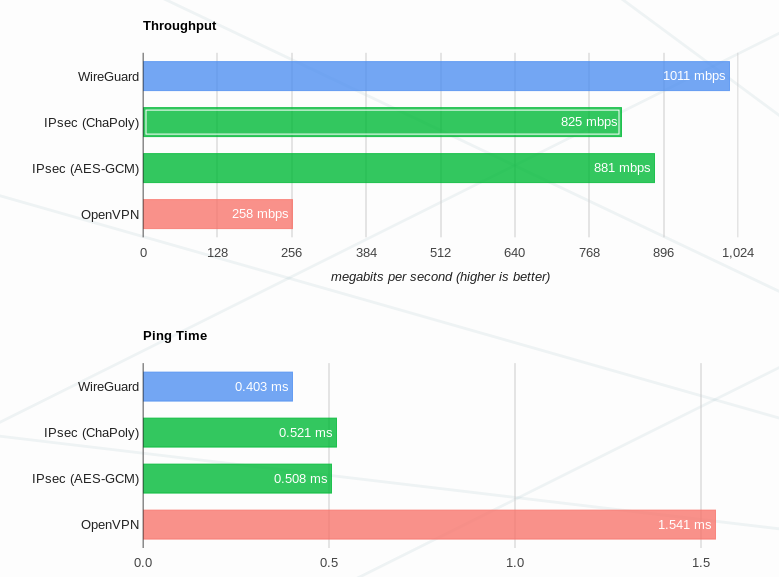
\includegraphics[scale=0.45]{img/wireguard_performance}
	\caption[Benchmark tra IPsec, OpenVPN e WireGuard]{Benchmark tra IPsec, OpenVPN e WireGuard.
		OpenVPN è la soluzione più lenta poiché è l'unica implementata in \textit{userspace}.
		\url{https://www.wireguard.com/performance/}}
	\label{fig:wireguard-performance}
\end{figure}
Un interfaccia WireGuard può gestire più peer, ed occorre che le chiavi pubbliche di tutti
i peer a cui ci si vuole connettere siano presenti su tutti i partecipanti.
WireGuard ha un grande potenziale, tuttavia è poco configurabile. Questo ha il vantaggio
di rendere tale soluzione molto facile da configurare, al prezzo di, semplicemente, avere
molte meno opzioni su cui intervenire. In fase di scelta
finale, questa soluzione è stata infine scartata perché funzionante su UDP.
	      
	      
	      
\subsection{IPsec/L2TPv3 e EtherIP/IPsec}
\begin{itemize}
	\item L2TP versione 3 è l'ultimo aggiornamento del protocollo L2TP, principalmente implementato in
	      device Cisco. Analogamento ad L2TP, è possibile usarlo per creare VPN LAN-to-LAN al livello 2.\\
	      Viene supportato dai principali produttori di apparati di rete, oltre che da Linux.
	\item EtherIP è un protocollo per l'incapsulamento di frame Ethernet in pacchetti IP, il cui scopo è quello
	      di connettere tra loro diverse LAN a livello 2.
\end{itemize}
Entrambi i due protocolli devono essere incapsulati in IPsec per ottenere una VPN che garantisca proprietà
di sicurezza.
EtherIP è
supportato da Linux e da SoftEther VPN Server.\\
Le due tecnologie sono in qualche modo simili, poiché realizzano connessioni a livello 2. Nel caso in cui
MoonCloud abbia esigenze di lavorare al livello 2, queste soluzioni sono da prendere in considerazione, sebbene
anche OpenVPN e SoftEther supportino VPN a questo layer.
	      
	      
\subsection{PPTP}
Il protocollo \textit{PPTP - Point To Point Tunneling Protocol} è un protocollo
\textit{legacy}, sviluppato da Microsoft e non più sicuro, sebbene (purtroppo)
ancora usato.
Questo protocollo offre VPN, ma non è assolutamente una soluzione praticabile per
MoonCloud.
